%************************************************
\chapter{Implementation}\label{ch:implementation}
%************************************************

This chapter gives an overview of the implementation aspects of the smartwatch controlled mobile music player. It explains the application structure, the chosen interaction techniques and the mobile-wear communication system.

The essential music library is provided by a private Spotify\footnote{Music streaming service: \url{www.spotify.com}} premium account. Spotify has a powerful and beneficial \ac{API} which adds useful meta data such as audio features to each track. Audio features are high-level acoustic attributes like tempo or valence which are used in a system for coarse track selection. The prototype is divided into two separate applications, i.e. mobile (handheld) and wear (smartwatch) application. Users are able to access all features of the mobile application via the smartwatch application. In order to cover a lot of different levels of the focused-casual continuum \cite{pohl2013focused}, three interaction techniques, differing in the amount of control granted, are available for the user:
\begin{itemize}
\item{Touch}
\item{Speech}
\item{Gesture}
\end{itemize}
Each technique can be used for the simpler actions of the music player such as play and pause, skip to previous or next song and changing the volume. However, for the more complex interactions, e.g. choosing a playlist, only the touch and speech interaction methods suffice since gestures for every playlist would be too hard to remember. Gesture and speech input can be performed casually while not even looking at the smartwatch. Section \ref{sec:UserInterface} describes the functionality and the power of the different methods.

\section{Hardware Requirements}\label{sec:hardwarerequirements}
Both applications are implemented for the android platform. The handheld device has no further hardware or software requirements other than supporting the android wearable \ac{API} for communicating with the smartwatch, thus a Samsung Galaxy S6 is chosen. The smartwatch application certainly requires the device to be equipped with a acceleration sensor and a microphone. A moto360 from Motorola is well suited for this. Both devices require Bluetooth functionality as well.

\section{Application Structure}\label{sec:ApplicationStructure}
The application is divided into two dedicated android applications, one for the mobile device and one for the smartwatch. Since the smartwatch has less computing power and battery life than a mobile device, all of the music players functionality is implemented in the mobile application where the Spotify Android \ac{SDK} for streaming functionality and the Spotify Web \ac{API} for Android\footnote{\url{https://github.com/kaaes/spotify-web-api-android}} for accessing the music information is used. Together they allow for every possible interaction with Spotify such as streaming music, creating playlists, searching for artists or tracks, etc. The wearable application provides an additional \ac{GUI} which contains the same information about the music arrangements as the mobile application's \ac{GUI} but with less overhead (e.g. images are not shown). It also is responsible for hosting the touch, speech and gesture input techniques. Figure \ref{fig:packageDiagram} shows each application's different components which are separated by java packages. Both applications consist of four packages:

\paragraph{Mobile Application}
The \textit{view} package contains the MainActivity of the application. It is responsible for both maintaining the \ac{GUI} elements (see section \ref{sec:UserInterface}) and turning issued commands into music player actions which are then forwarded to the SpotifyManager class. The \textit{speechcontrol} package contains the tool which interprets a speech command sent from the wearable application. See section \ref{sub:speechControl} for a detailed description about speech commands. The \textit{core} package contains both the CommunicationManager class that handles messaging between wearable and mobile application and the SpotifyManager class which ties the Spotify Android \ac{SDK} and the Spotify Web \ac{API} for Android together. On the application start it downloads information about the music items that belong to the logged in Spotify account and serves it to the \ac{GUI}. Audio features are downloaded for each track in the user's library as well. They are stored in the AudioFeatureDatabase class in form of a Hashmap with the track's id as key and a list of the audio features as the value. The AudioFeatureDatabase class is also responsible for searching tracks from the library with a specified audio feature value (section \ref{sub:speechControl} describes why this is useful and how it works). Audio features are also saved to the mobile phones disk by the SpotifyCache class to reduce the amount of data that has to be downloaded on the application start.

\paragraph{Wearable Application}
The wearable application's structure is similar to the mobile application. Classes responsible for maintaining the \ac{GUI} elements are located in the \textit{view} package. The \textit{wiigee} package contains a pre-built event driven library for acceleration based gesture recognition (see section \ref{sub:gestureControl} for further details). The \textit{core} package contains the CommunicationManager that again is responsible for messaging between wearable and mobile application. Also the system for recording speech and transforming it into text is located in the \textit{core} package. As soon as voice recognition is enabled (see section \ref{sub:speechControl}) the VoiceRecognitionListener class receives the recognized text from android's Speech Recognizer and waits until the final keyword is included. The text is then sent to the mobile application to be interpreted.


\begin{figure}[bth]
	\myfloatalign
	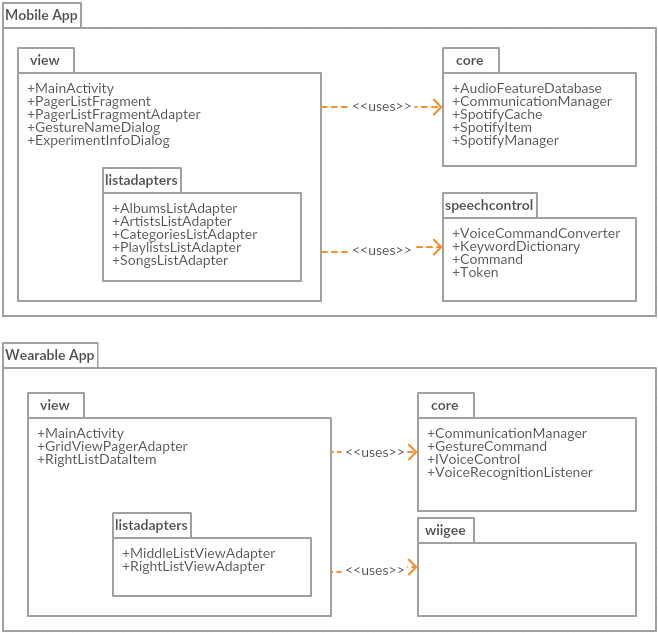
\includegraphics[width=1\linewidth]{img/PackageDiagramCombined.png}
	\caption{Package diagram of the mobile (top) and wearable (bottom) application.}
	\label{fig:packageDiagram}
\end{figure}

\section{User Interface}\label{sec:UserInterface}
The \ac{GUI} from the mobile application only differs from the wear \ac{GUI} in terms of unimportant information such as images. In terms of control over the music player, both versions offer the same possibilities and show the synchronized player state (when connected) at any given time. The wear application, however, additionally introduces speech and gesture interactions which the mobile application is not capable of.

It is noteworthy that the Spotify \ac{SDK} offers a lot more functionality than implemented, such as creating own playlists or searching the entire Spotify music library for keywords. The implemented music player, however, just offers the basic playback functionalities in order to keep the application simple and to not overload the participants in the experiment with information since they have to remember how to control the music player. Moreover, more music player functions would not have an impact on the experiment results.

\subsection{Touch Input - \ac{GUI}}
Both \ac{GUI}s are designed to be simple and straightforward. The mobile version mainly consists of two areas. Figure \ref{fig:mobileGUI} depicts a screenshot of this layout. A control panel is situated at the bottom of the screen. Above this is a left-right scrollable pager containing different kinds of lists. \marginpar{Categories are Spotify's extended version of genres} The scrollable list pager\footnote{A horizontal scrollable container holding vertical scrollable lists.} contains five lists, one for each music arrangement which are playlists, songs, albums, artists and categories.
\begin{figure}[bth]
	\myfloatalign
	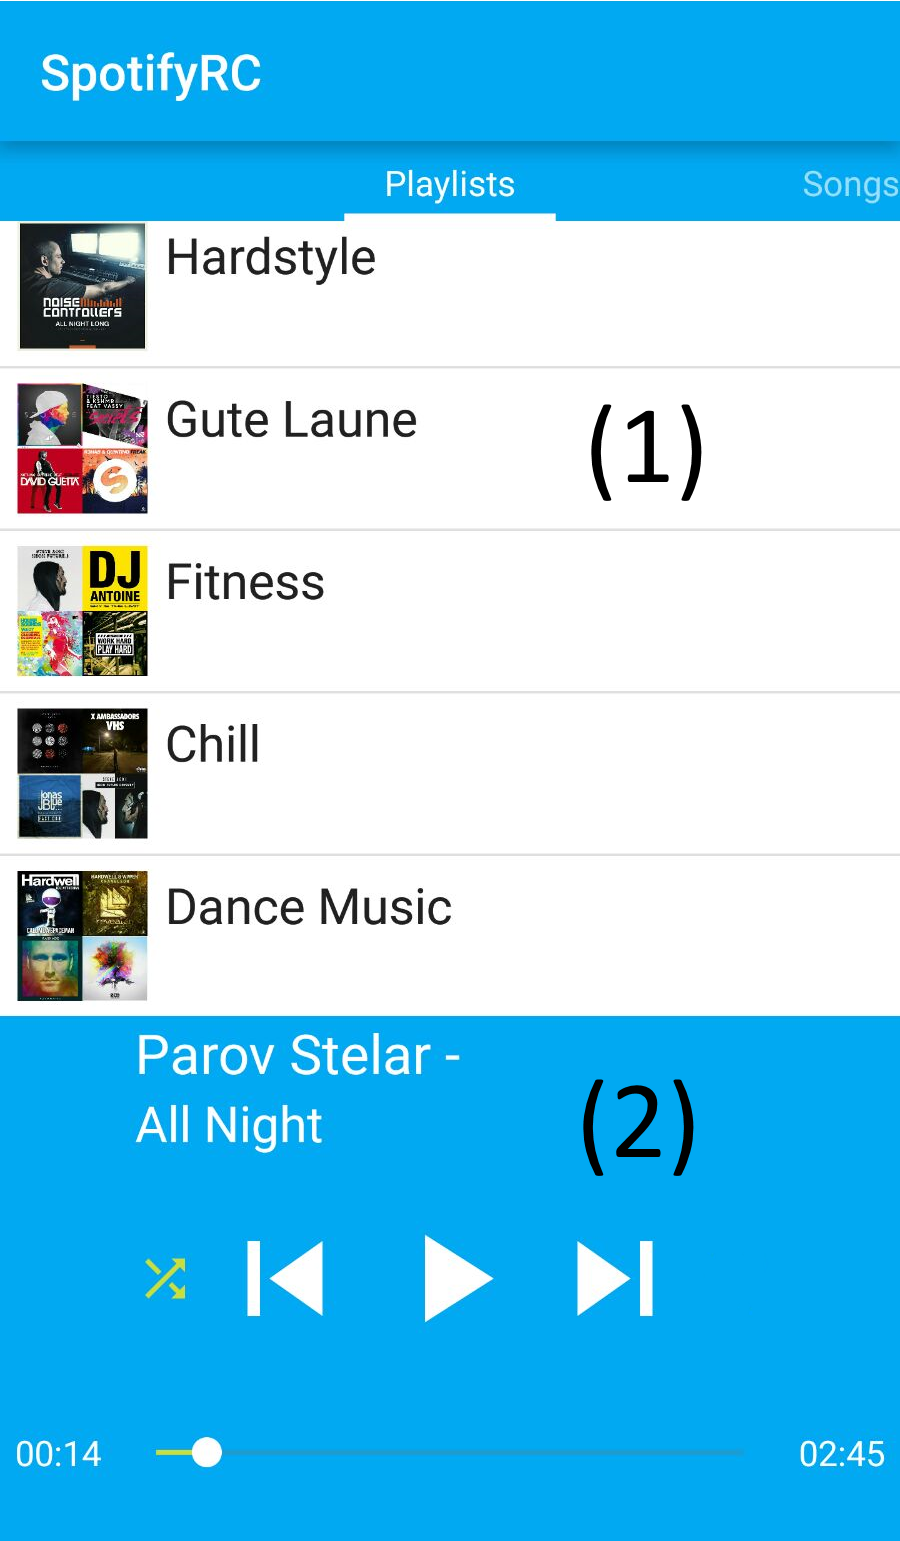
\includegraphics[width=.45\linewidth]{img/mobileGUIlabeled.png}
	\caption{\ac{GUI} of the mobile application. (1) shows the left-right scrollable list pager with indicators which list is shown at the top. (2) shows the player control panel in blue.}
	\label{fig:mobileGUI}
\end{figure}
The control panel located beneath the list pager contains four control buttons such as a shuffle button including on-off indicator, a skip to previous song button, a play-pause button and a skip to next song button. Unlike the wear application, the mobile version spares buttons for controlling the volume, because most devices own hardware buttons for this purpose. Information on the name of the current song and artist can be found above these buttons. The track's progress and total duration can be found at the very bottom of the screen. \\

However, the intention of the wear application is, that the user does not need to bother reaching his mobile phone. For this reason, the wear application's \ac{GUI} offers the same amount of control over the music player via its touch input. Figure \ref{fig:wearGUI} demonstrates the layout of the wear application. It consists of a GridViewPager\footnote{A grid based omni-directional scrollable container holding views} with one row and three horizontal pages (columns). 

\begin{figure}[bth]
	\myfloatalign
	\subfloat[control panel in interactive mode]
	{\label{fig:wearGUI-controls}
	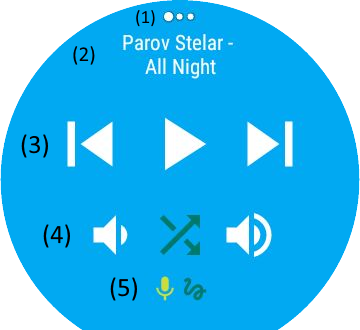
\includegraphics[width=.3\linewidth]{img/wearGUIcontrolsPage.png}} \quad
	\subfloat[list of music arrangements]
	{\label{fig:wearGUI-select}
	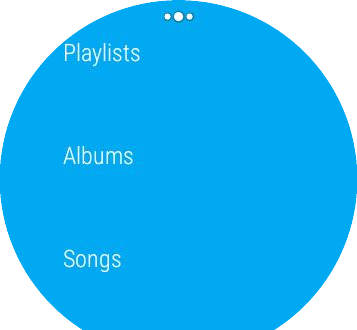
\includegraphics[width=.3\linewidth]{img/wearGUIselect.png}} \quad
	\subfloat[list of playlists]
	{\label{fig:wearGUI-items}
	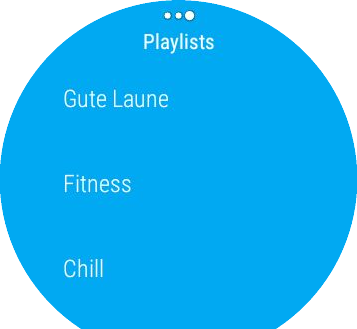
\includegraphics[width=.3\linewidth]{img/wearGUIitems.png}} \\
	\subfloat[control panel in ambient mode]
	{\label{fig:wearGUI-ambient}
	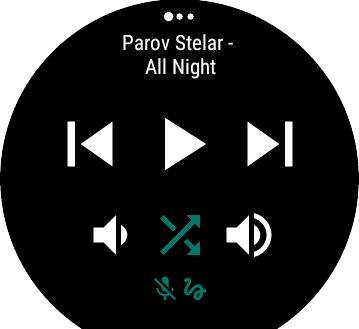
\includegraphics[width=.3\linewidth]{img/wearGUIambient.png}}
	\caption{ The \ac{GUI} of the wear application consists of a GridViewPager containing three horizontal pages. A dot indicator at the top of the screen shows the current page. \ref{fig:wearGUI-ambient} depicts the controls page in ambient mode, i.e. battery saving mode, while \ref{fig:wearGUI-controls} is the same screen in interactive mode. Swiping right brings up the list of music arrangements \ref{fig:wearGUI-select}. Selecting e.g. playlists switches to the third page \ref{fig:wearGUI-items} showing a list with all playlists.}
	\label{fig:wearGUI}
\end{figure}

Figure \ref{fig:wearGUI-controls} shows the main control page which is divided into five rows (1) - (5). A dot indicator showing the current page with a bigger dot is located at the top of the screen in row (1). Row (2) contains the current artist and track that is playing. Row (3) and (4) contain the control buttons, i.e. in (3) the buttons for play previous song, toggle play and pause, play next song and in (4) the buttons for decrease volume, toggle shuffle (grey = off, green = on) and increase volume are located. Row (5) contains two icons which indicate whether speech and gesture recognition are active (green) or inactive (grey).

Figure \ref{fig:wearGUI-select} shows the page in the middle which is reached by swiping over the screen from right to left. The page contains a vertical scrollable list of the five music arrangements, namely playlists, songs, albums, artists and categories. Selecting a list entry scrolls to the right (the third) page which always adapts its list showing the respective items in the selected arrangement. \\

The moto360 smartwatch is equipped with a battery saving mode called ambient mode. In this mode cpu processing is reduced and it is recommended\footnote{\url{https://developer.android.com/training/wearables/apps/always-on.html}} to reduce the \ac{UI} layout to a black background and white text color. Updates to the \ac{UI} should then happen on a several seconds up to a minute basis. Applications that run in both ambient and interactive mode are called \textit{always-on apps}. The transition from interactive to ambient mode happens either automatically after a short period of user inactivity or can be forced by covering the screen. Leaving ambient mode happens either by touching the screen or by bringing up the wrist as in looking at the time. Figure \ref{fig:wearGUI-ambient} depicts the control page of the wear application running in ambient mode with a black background and white text and icon color. \\

\subsection{Speech Control}\label{sub:speechControl}
The wear application offers the possibility to control the music player via speech commands. In order to enter a speech command, the application must be in interactive mode which activates the continuous speech recognition (indicated by the green microphone seen in \ref{fig:wearGUI-controls} at the bottom of the screen). The user can then talk to the watch and issue a command. Speech data is recorded and converted to text by the android speech recognition service\footnote{\url{https://developer.android.com/reference/android/speech/SpeechRecognizer.html}}. Since the speech recognition happens continuously input must be recognized easily as a possible valid command. Therefor every command has to end with a special final keyword, the word \textit{``bitte''}\marginpar{``Bitte'' is the german word for ``please''}. As soon as the wear application detects this keyword, the converted text is send to the mobile application where it gets parsed, transformed into a command and finally executed. Figure \ref{fig:speechActivityDiagram} illustrates this procedure with an activity diagram. The wear-mobile communication process is described in more detail in section \ref{sec:Communication}.
\begin{figure}[bth]
	\myfloatalign
	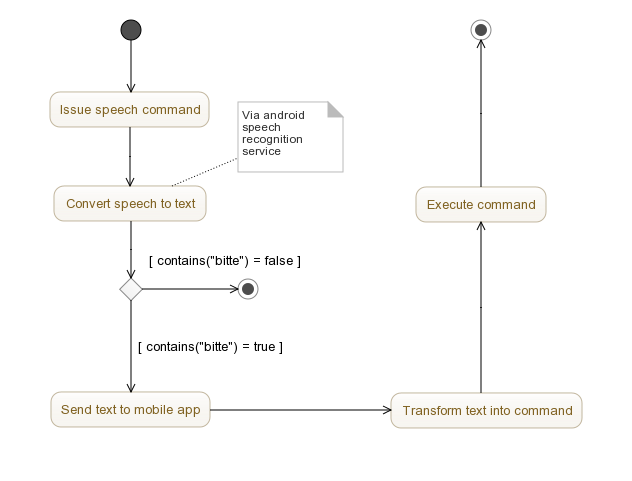
\includegraphics[width=1\linewidth]{img/SpeechActivityDiagram.png}
	\caption{Activity diagram of the speech interaction procedure. Actions to the left of the dashed line happen in the wear application and actions to the right of the dashed line happen in the mobile application. At stage (1) a preliminary decision is made whether the converted text resembles a command or not.}
	\label{fig:speechActivityDiagram}
\end{figure}

In order to cover the focused-casual continuum speech commands for this music player are divided into three groups based on their power and complexity. The first group contains the simplest commands that just consist of one keyword. Commands in the second group start with a keyword and are followd by additional words, until the final keyword occurs, that are handled as the input parameters. Commands in the third group are built by chaining different keywords together forming a simple sentence.

Table \ref{tab:speechCommands} contains the respective keywords for commands in the first two groups. The first six simple keywords each represent a command by itself and thus belong to group 1. The \textit{play} command is the only command in group 2 meaning it requires a parameter to work as intended.

\begin{table}[bt]
	\myfloatalign
	\begin{tabularx}{\textwidth}{XX} \toprule
		\tableheadline{Speech Command Keywords} & \tableheadline{Actions in Music Player} \\ 
		\midrule
		pause & pause music playback \\
		weiter & resume music playback \\
		n\"achstes & skips to next song \\
		zur\"uck & skips to previous song \\
		lauter & increases the volume \\
		leiser & decreases the volume \\
		\midrule
		play <music element> & load and play an element from the music library \\
		\bottomrule
	\end{tabularx}
	\caption{Speech commands from the first two groups. The play command is the only command accepting parameters. All other commands in this table belong to group 1. To issue a command, simply activate speech recognition by entering the watches interactive mode and say the keyword followed by the final keyword ``bitte''.}
	\label{tab:speechCommands}
\end{table}

Commands in the third group, which are built by chaining the keywords shown in table \ref{tab:speechCommandsAudioFeature} together, offer a special kind of control over the music player. They allow for queuing and playing tracks that differ in terms of an audio feature from the current playing track. This enables users to change the type of music in contexts not allowing for high engagement.

\begin{description}
	\item[Audio Feature:] Spotify runs a suite of audio analysis algorithms on every track in their catalog. These extract about a dozen high-level acoustic attributes from the audio. Some are well-known musical features, like tempo and loudness. Others are more specialized, like valence and energy.
\end{description}

The four most intuitive audio features are supported by the music player to be used with speech commands, which are\footnote{A complete list of audio features and their meaning can be found at: \url{https://developer.spotify.com/web-api/get-several-audio-features/}}:
\begin{description}
	\item[Tempo:]The estimated tempo of a track measured in \ac{BPM}. It derives directly from the average beat duration.
	\item[Energy:]A measure from 0.0 to 1.0 and represents a perceptual measure of intensity and activity. Typically, energetic tracks feel fast, loud, and noisy. For example, death metal has high energy, while a Bach prelude scores low on the scale.
	\item[Loudness:]The overall loudness of a track in decibles (dB). Loudness values are averaged across the entire track. Loudness is the quality of a sound that is the primary psychological correlate of physical strength (amplitude). Values range between -60 and 0 db.
	\item[Valence:]A measure from 0.0 to 1.0 describing the musical positiveness conveyed by a track. Tracks with high valence sound more positive, while tracks with low valence sound more negative.
\end{description}

\begin{table}[h]
	\myfloatalign
	\begin{tabularx}{\textwidth}{XXX} \toprule
		\tableheadline{Scaling} & \tableheadline{Direction} & \tableheadline{Audio Feature} \\ 
		\midrule
		etwas & mehr & Tempo \\
		viel & weniger & Energie \\
		 & & Lautst\"arke \\
		 & & Stimmung \\
		\bottomrule
	\end{tabularx}
	\caption{Building blocks (keywords) for commands from the third group. Choose a keyword from each column, chain them to a sentence and attach the final keyword ``bitte'' at the end. The scaling keyword can be omitted.}
	\label{tab:speechCommandsAudioFeature}
\end{table}

Changing tracks based on the current track's audio features enables the user to specify what kind of music she wants to listen to without deciding on the exact tracks to be played in a situation where high engagement is not possible. The pseudo code in listing \ref{lst:audioFeature} is responsible for searching the corresponding tracks in the music library. The new value for the specified audio feature is calculated in line 2 respectively 4 by first evaluating the direction keyword which determines whether to increase or decrease the current value. The scale keyword then determines the scaling factor which indicates by how much the current value is changed. Therefor the scaling factor is multiplied by the distance between the current value and either the global minimum or maximum value for the given audio feature depending on the direction keyword. Afterwards, tracks in  range of the new calculated value, determined by a tolerance radius, are searched (line 7 and forth). The tolerance radius is increased by a fix amount as long as no tracks are found. Figure \ref{fig:audioFeatureExample} explains this mechanism with example values.

\begin{lstlisting}[caption=Pseudo code for calculating the new audio feature value and looking up respective tracks with a tolerance radius from the music library, label=lst:audioFeature]
if(direction == negative) {
	newValue = cur + (cur - min) * -scale;
} else {
	newValue = cur + (max - cur) * scale;
}

while(noTracksFound) {
	lookupTracksWithValueAndTolerance(newValue, tolerance);
	increase(tolerance);
}
\end{lstlisting}

\begin{figure}[bth]
	\myfloatalign
	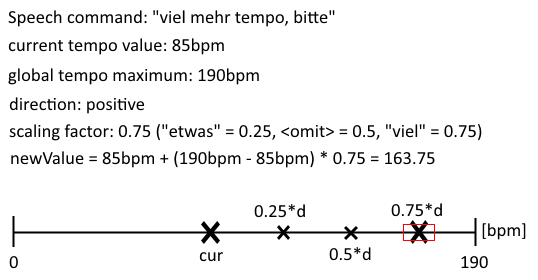
\includegraphics[width=.7\linewidth]{img/calcAudioFeatureExample.png}
	\caption{Example calculation for changing tracks based on the audio's tempo. The big X's show the current and the new value, while the smaller ones depict values with a smaller scaling factor. The red rectangle around the new value illustrates the tolerance radius in which new tracks are searched.}
	\label{fig:audioFeatureExample}
\end{figure}

After sending a possible speech command to the mobile application, the text needs to be converted to an applicable command. For this, a conversion algorithm first searches the text for command keywords from the first two speech command groups (see table \ref{tab:speechCommands}) and creates a token of a respective type for it when found. Tokens that belong to the simple commands in the first group are directly mapped to their corresponding music player command and then executed. 

In case the text contains a \textit{play} keyword which is followed by at least one word, an additional token is created for it, being the parameter of the command.\marginpar{Item names of songs and albums are a combination of their name and the artist} The algorithm then tries to find the desired music library item by comparing the item name with the parameter text. Because item names often contain additional artifacts, such as \textit{Radio Edit} or \textit{Original Mix}, and the speech to text conversion is not always accurate, comparison is not based on equality but rather on similarity. The pseudo code in listing \ref{lst:stringSimilarity} finds the item name with the highest similarity to the parameter text based on the \textit{Levensthein distance}\footnote{String metric for measuring the number of required edits in one string in order to match the other.}. An item name which equals the parameter text can be considered as most similar. However, in case the item name is longer than the command's parameter, the foreach loop starting in line 7 computes the minimum distance for every substring of the item name with the same length of the parameter. In the end, the item with the minimum distance which is equal to the highest similarity to the parameter is returned and played.

\begin{lstlisting}[caption=Calculating parameter and music item name similarity, label=lst:stringSimilarity][Ht]
var mostSimilarItem = null;
foreach(item in library) {
  if(parameter == item.name) { 
    return item; //distance is already 0, so we found the item
  }
  var minDistance = Integer.MAX;
  foreach(substring s of item.name with s.length == parameter.length) { //if the parameter is longer than the item name, only one iteration happens
    distance = Levensthein(parameter, s);
    if(distance < minDistance) { 
      minDistance = distance; //less distance = higher similarity
      mostSimilarItem = item;
    }
  }
}
return mostSimilarItem;
\end{lstlisting}

If no keywords for group 1 or 2 are found, the conversion algorithm checks for keywords belonging to the third group and creates a token for each one. The text is a valid command if at least a token for the direction and the audio feature is present. A scaling keyword can be omitted and the order of the tokens is not considered. The tokens are then used to directly set the parameters of the formula for calculating the new value for the specified audio feature (see listing \ref{lst:audioFeature}).\\

The following commands are examples from every group executed on the music library from a private spotify account:
\begin{description}
	\item[1. ``n\"achstes, bitte'':] skips to the next song in the queue
	\item[2. ``play Hardwell, bitte'':] enqueues and plays all tracks by Hardwell from the library
	\item[3. ``viel mehr Tempo, bitte'':] plays tracks from the library with significantly increased tempo compared to the current
\end{description}

% http://venturebeat.com/2015/05/28/google-says-its-speech-recognition-technology-now-has-only-an-8-word-error-rate/ use in evaluation chapter!
% how to bibtex webpages:
% @misc{WinNT,
%  title = {Google says its speech recognition technology now has only an 8% word error rate},
%  howpublished = {\url{http://web.archive.org/web/20080207010024/http://www.808multimedia.com/winnt/kernel.htm}},
%  note = {Accessed: 2010-09-30}
%}

\subsection{Gesture Control}\label{sub:gestureControl}
The third interaction technique supported by the implemented music player involves acceleration based gesture recognition. With this the user is able to issue commands to the player without looking at or touching the screen with the other hand. Gesture commands on the contrary are not as powerful as touch input or speech commands. They only offer control for pause and resume, skip to next song, back to previous song as well as increase and decrease volume. The other commands that speech input offers would result in gestures too complex to perform and remember for a user\cite{kuhnel2011m}.

For this, a pre-built event-driven gesture recognition library called \textit{Wiigee}\footnote{Official Wiigee site: \url{www.wiigee.org}} is used. Wiigee accepts three dimensional acceleration vectors as input for pattern training and recognition. The vectors are sent through a four-level recognition pipeline which is shown in Figure \ref{fig:wiigeePipeline}. \cite{Schlomer:2008:GRW:1347390.1347395} describe the four stages of this classical recognition pipeline in detail. They observed an average rate of correctly recognized gestures of 90\%. 

\begin{figure}[bth]
	\myfloatalign
	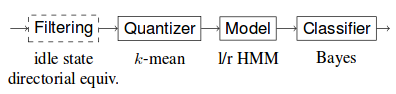
\includegraphics[width=1\linewidth]{img/wiigeePipeline.png}
	\caption{Original from \cite{Schlomer:2008:GRW:1347390.1347395}. Four-level recognition pipeline that first filters vector data und clusters it using a k-means algorithm. Subsequently a hidden markov model is fed with the clustered data and classified by a Bayesian classifier.}
	\label{fig:wiigeePipeline}
\end{figure}

In order to recognize gestures, they first have to be trained to wiigee. For later use, the data for every gesture can be saved to a file afterwards. \cite{Schlomer:2008:GRW:1347390.1347395} claims that a training session with five to ten repetitions is sufficient for Wiigee to learn a new gesture. The gestures for controlling the music player are kept short, simple and symbolic as \cite{kuhnel2011m} suggests. However, to avoid unintentional commands and to save battery life, an activation gesture has to be performed beforehand. Also, Wiigee does not support continuous gesture recognition. Figure \ref{fig:gestures} shows a list of all supported gestures and their meaning including the activation gesture. 

Once Wiigee recognized a gesture it notifies the registered listeners sending the recognized gesture id and a confidence score between 0 and 1. In order to filter out false positives, the confidence score has to exceed 0.97 before the gesture is accepted by mapping its id to a music player command.

\begin{figure}[h]
	\myfloatalign
	\subfloat[Activation gesture]
	{\label{fig:gesturesActivation}
	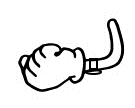
\includegraphics[width=.25\linewidth]{img/activationgesture.png}} \quad
	\subfloat[swipe arm from left to right: skip to next song]
	{\label{fig:gesturesNext}
	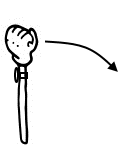
\includegraphics[width=.25\linewidth]{img/next.png}} \quad
	\subfloat[swing arm upwards: increase volume]
	{\label{fig:gesturesVolumeup}
	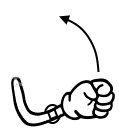
\includegraphics[width=.25\linewidth]{img/volumeup.png}} \\
	\subfloat[punch forward: play and pause]
	{\label{fig:gesturesPlaypause}
	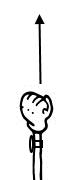
\includegraphics[width=.25\linewidth]{img/playpause.png}} \quad
	\subfloat[swipe arm from right to left: back to previous song]
	{\label{fig:gesturesPrevious}
	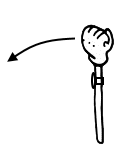
\includegraphics[width=.25\linewidth]{img/previous.png}} \quad
	\subfloat[swing arm downwards: decrease volume]
	{\label{fig:gesturesVolumedown}
	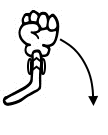
\includegraphics[width=.25\linewidth]{img/volumedown.png}}
	\caption{\ref{fig:gesturesActivation} depicts the activation gesture where the arm is bent and the watch face is turned down until the pitch threshold is reached. When the vibration countdown is over, one of the other five gestures can be performed to issue a command to the music player.}
	\label{fig:gestures}
\end{figure}

The activation gesture is performed by rotating the watch with its face down reaching a pitch of at least -70\textdegree or lower. For this, the rotation of the watch is constantly measured with android's software-based \textit{Game Rotation Vector Sensor}\footnote{Documentation can be found here: \url{https://developer.android.com/guide/topics/sensors/sensors_position.html}}. When the gesture recognition gets activated, the user receives a sequence of three vibrations as feedback from the watch after which a gesture can be performed. Wiigee's recognition algorithm is sensitive to the device rotation, hence the device orientation during recognition should be approximately the same as it was during the training in order to be recognized correctly.

Since it can not be assumed that users wear their watch in the same position and certainly have different wrist anatomies, a suited pitch value for the activation gesture has to be determined. An informal experiment involving 26 participants has been conducted, where each participant had the task to turn their wrist five times as much as possible without getting uncomfortable. The minimum values from each participant series are plotted in figure \ref{fig:pitchPlot}.

\begin{figure}
	\myfloatalign
	\begin{tikzpicture}
		\begin{axis}[
			width=\linewidth,
			xlabel=Participant No.,
			ylabel=Pitch in degree,
			ybar,
		]
		\addplot
		table[x=number,y=pitch, col sep=comma]{data/minPitchValues.csv};
		\end{axis}
	\end{tikzpicture}
	\caption{Minimum absolute pitch values for each participant. The minimum absolute pitch value that every participant reached is 70.3}
	\label{fig:pitchPlot}
\end{figure}

Wiigee is an event-based library where the training and recognition process is started by virtual button presses and completed by virtual button releases. In case of the Wiimote\footnote{Wiimote is a remote controller for the Nintendo Wii}, for which wiigee was originally designed, users were able to press real buttons. Gesture recognition on the smartwatch, however, can not be activated by real buttons, therefor training and recognition are activated by a virtual button press which is send to wiigee after the vibration countdown from the activation gesture. The virtual button release for finishing the training or recognition process is send automatically to wiigee after 750ms, which is enough time to perform each gesture. Deactivating the recognition process as soon as the device stops moving could not be used in this case, since this event can not be reliably detected.
\newpage
\section{Mobile-Wear Communication}\label{sec:Communication}
Controlling the music player with the smartwatch requires some communication to happen between the watch and the mobile device. Android provides a solution for this which is called the Wearable Data Layer \ac{API}\footnote{\url{https://developer.android.com/training/wearables/data-layer/index.html}} that is part of Google Play Services. It offers a communication channel for smartphone and wearable applications. In particular, the \textit{MessageApi} class which is responsibule for sending text messages back and forth suffices for the music player. A message can have different types determined by a string that has to be attached to the message. Table \ref{tab:messageTypes} lists all types that can be attached to a message in both the wearable and mobile application as well as their purpose and when they are sent. Figure \ref{fig:communicationoverview} illustrates in which direction the messages are sent.

\begin{figure}[bth]
	\myfloatalign
	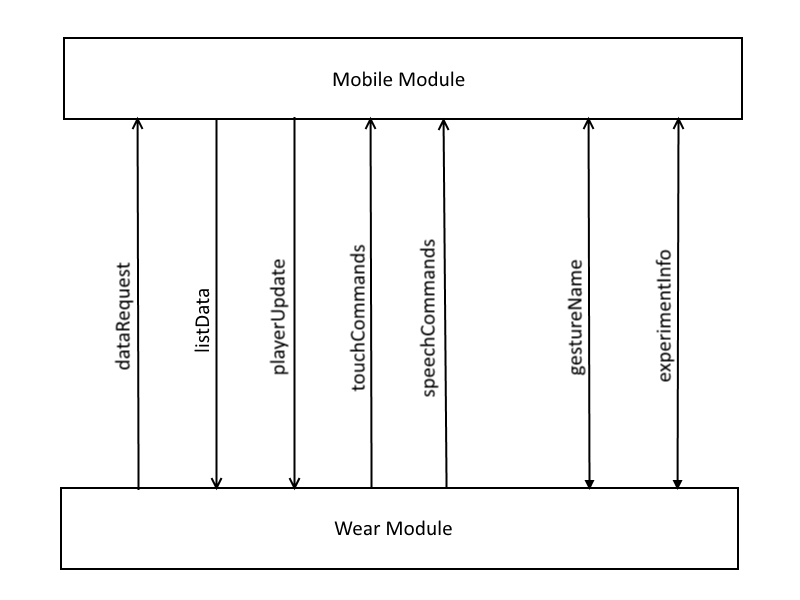
\includegraphics[width=1\linewidth]{img/CommunicationOverview.png}
	\caption{A Message can be of five different types: a data request type, list data type containing information about the music library, an update type containing the current music player state, a touch command type and a speech command type which both are sent from the wearable application and answered by the mobile application afterwards. The two greyed out message types on the right are included for the sake of completeness and are only used for the user study.}
	\label{fig:communicationoverview}
\end{figure}

A communication manager class in both applications is responsible for sending and receiving these messsages. When a message is received, the communication manager forwards the message to the  concerned application parts which then execute a corresponding action.

\begin{table}[h]
	\myfloatalign
	\begin{tabularx}{\textwidth}{XXX} \toprule
		\tableheadline{Message Type} & \tableheadline{When Sent} & \tableheadline{Purpose} \\ 
		\midrule
		data request & wear app start. & Indicates the mobile app that music library data is needed. \\
		list data & mobile app start or when a data request was received. & Contains a list of display names for all music items in the library. \\
		update & on music player's state change, i.e. when the track is changed, a play or pause command ocurred or shuffle was toggled. & Contains all information to keep mobile and wear \ac{UI} synchronized. \\
		touch command & on touch or gesture input on the wear app. & Contains a string representation of the issued command. A gesture id is mapped to the same string as its respective touch command is (see \ref{sub:gestureControl}). \\
		spech command & after user completed a speech command & Recorded text is sent to the mobile app to convert it into a command \\
		\bottomrule
	\end{tabularx}
	\caption{List of the different message types, when they are sent and what their content or purpose is.}
	\label{tab:messageTypes}
\end{table}


%Chapter \ref{ch:implementation} 


%*****************************************
%*****************************************
%*****************************************
%*****************************************
%*****************************************




